% !TEX root = ../intro-stellar-physics.tex

\nocite{Mihalas1978Stellar-Atmosph,LeBlanc2010An-Introduction,Carroll2006An-Introduction}

\section{The Boltzmann Equation}
\label{s.boltzmann-eqn}

Suppose we have a sample of atoms, all of the same species.  The electrons in those atoms can be in any number of energy levels; we'll denote the energy of level $n$ as $E_{n}$.  There may be many different states with the same energy; we'll denote the total number of possible states\sidenote{Known as the \emph{degeneracy} of a given energy} with energy $E_{n}$ as $g_{n}$.  For example, in a neutral hydrogen atom, the energy and degeneracy of level $n$ are
\begin{eqnarray*}
 E_{n} &=& \val{13.6}{\eV}\left(1-\frac{1}{n^{2}}\right)\\
 g_{n} &=& 2n^{2}.
\end{eqnarray*}
Here the ground state has $n = 1$ and $E_{1} = \val{0}{\eV}$.

The basic principle of statistical (thermal) physics is that if our sample is in thermal equilibrium, then the ratio of the number of atoms in state $i$ to the number in state $j$ is
\begin{equation}\label{e.boltzmann}
\frac{N_{i}}{N_{j}} = \frac{g_{i}}{g_{j}} 
\exp\left(-\frac{E_{i}-E_{j}}{\kB T}\right).
\end{equation}
Suppose we wish to know the fraction of atoms in a given state $i$: that is, we want to know
\[	x_{i} = \frac{N_{i}}{N_{1}+N_{2}+\ldots+N_{i}+\ldots} ? \]
Using equation~(\ref{e.boltzmann}), we can express $x_{i}$ as 
\begin{eqnarray}
  x_{i} &=& \frac{N_{i}/N_{1}}{1+N_{2}/N_{1}+\ldots+N_{i}/N_{1}+\ldots}\nonumber\\
        &=& \frac{g_{i}e^{-E_{i}/\kB T}}{g_{1}e^{-E_{1}/\kB T}+g_{2}e^{-E_{2}/\kB T}+\ldots+g_{i}e^{-E_{i}/\kB T}+\ldots} \nonumber\\
        &\equiv& \frac{g_{i}e^{-E_{i}/\kB T}}{\pfcn}.
\end{eqnarray}
The quantity 
\[ \pfcn = \sum_{i} g_{i}\exp\left(-\frac{E_{i}}{\kB T}\right) \]
is called the \emph{partition function}: loosely speaking, it indicates the number of ways the sample of atoms can be partitioned among the different energy levels.

\begin{exercisebox}[Partition function for neutral hydrogen]
For a neutral hydrogen atom, what is the limit of $\pfcn_{\mathrm{H}}(T)$ for $\kB T \ll \val{13.6}{\eV}$?  How does $\pfcn_{\mathrm{H}}(T)$ qualitatively change with temperature: does it increase, decrease, or something else?
\end{exercisebox}

\section{Ionization: The Saha equation}
\label{s.saha-eqn}

As the temperature in the gas rises, collisions between atoms become sufficiently energetic to eject electrons from atoms.  In astronomy, the ionization state is denoted by a small Roman numeral: Fe\,\textsc{i} denotes neutral iron, Fe\,\textsc{ii} denotes singly-ionized iron, Fe\,\textsc{iii} denotes doubly-ionized iron, and so on. We'd like to extend equation~(\ref{e.boltzmann}) to find the ratios of two ionization states $N\,(i+1)/N\,(i)$.  There are some complications, however, and deriving this ratio is beyond the scope of this course. What we will do is look at the equation for this ratio, known as the \emph{Saha equation}, and try to understand how it works.  The Saha equation for the ratio of ionized to neutron hydrogen is
\begin{equation}\label{e.saha}
\frac{N\,\textrm{\scshape ii}}{N\,\textrm{\scshape i}} 
= {\color{red}\left[\frac{2}{n_{e}}
\left(\frac{2\pi m_{e}kT}{h^{2}}\right)^{3/2}\right]}
\frac{\pfcn_{\mathrm{II}}}{\pfcn_{\mathrm{I}}} \exp\left(-\frac{E_{\mathrm{ion}}}{\kB T}\right).
\end{equation}
In this equation, $n_{e}$ denotes the electron density---the number of free electrons per unit volume---and $m_{e}$ is the electron mass.

Let us interpret equation~(\ref{e.saha}) in terms of eq.~(\ref{e.boltzmann}).  First, there is the factor $\exp(-E_{\mathrm{ion}}/\kB T)$. Here $E_{\mathrm{ion}}$ is the difference in energy between the ground states of the different ionization stages (for this example, $E_{\mathrm{ion}} = \val{13.6}{\eV}$).  That is just as in equation~(\ref{e.boltzmann}). To understand the factor $\pfcn_{\mathrm{II}}/\pfcn_{\mathrm{I}}$, consider that we are asking for the ratio between the total number of ionized atoms to the total number of neutral atoms; and this means summing over all of the states with electrons in different energy states. It is plausible, therefore, that the factor $g_{i}/g_{j}$ from equation~(\ref{e.boltzmann}) would be replaced by $\pfcn_{\mathrm{II}}/\pfcn_{\mathrm{I}}$.

In addition to the number of possible states for the ion, we need to allow for the number of possible electron states.  When the atom is ionized, each electron quickly acquires an average kinetic energy $(3/2)\kB T$. There are many different states with this energy: the electron can be in different locations, and moving in different directions.  At first, you might think that there would be an infinitude of possible electron states.  Quantum mechanics, however, sets limitations on the number of electron states.

First, we have the Pauli exclusion principle: no two electrons can be in the same location with the same momentum and same spin. What do we mean by same location and momentum?  Recall the Heisenberg uncertainty principle: the electrons $x$-position and $x$-momentum are spread about a range of values $\Delta x$ and $\Delta p_{x}$, and these uncertainties are related via
\[ \Delta x\,\Delta p_{x} \gtrsim h. \]
Thus, if we imagine dividing our volume into little boxes of volume
\[ 
 \Delta V = \Delta x\,\Delta y\,\Delta z \approx \frac{h^{3}}{\Delta p_{x}\,\Delta p_{y}\,\Delta p_{z}},
\]
each box can hold two electrons.\sidenote{Because electrons have spin 1/2, we can put two electrons into the same position and momentum state if their spins are oppositely directed.} Suppose we have a volume $V$; how many boxes are there?  The number of available boxes is
\[
	\frac{V}{\Delta V} \approx \frac{V\;\Delta p_{x}\,\Delta p_{y}\,\Delta p_{z}}{h^{3}}.
\]
To estimate the size of $\Delta p_{x}\,\Delta p_{y}\,\Delta p_{z}$, let's estimate $\Delta p_{x}\sim p_{x}$; further, if everthing is isotropic then $p_{x}\approx p_{y}\approx p_{z}$ on average, so $\Delta p_{x}\,\Delta p_{y}\,\Delta p_{z} \sim p_{x}^{3}$.  Now the kinetic energy of the electron is $p^{2}/2m_{e}$, and $p^{2} = p_{x}^{2} + p_{y}^{2} + p_{z}^{2} \approx 3 p_{x}^{2}$. Hence the kinetic energy is $(3/2)p_{x}^{2}/m_{e}$; in thermal equilibrium, however, the kinetic energy has an average value of $(3/2)\kB T$.  The value of $p_{x}^{2}$ is therefore
\[
	p_{x}^{2} \approx m_{e}\kB T,
\]
and the number of boxes is
\[
	\frac{V}{\Delta V} \sim V\frac{p_{x}^{3}}{h^{3}} \sim V\frac{\left(m_{e}\kB T\right)^{3/2}}{h^{3}}.
\]
If our volume $V$ contains $N_{e}$ electrons, then the number of boxes---which is the number of states---per electron is
\[
	\frac{2V}{N_{e}\Delta V} \sim \frac{2V}{N_{e}}\frac{\left(m_{e}\kB T\right)^{3/2}}{h^{3}}.
\]
The factor of 2 appears because each box can hold 2 electrons.  Recognizing that $N_{e}/V = n_{e}$, we see that this number of states per free electrons corresponds to the factor in $\color{red}\left[\;\right]$ in equation~(\ref{e.saha}). When the numerical calculation is done correctly, the additional factor of $2\pi$ arises.

\section{Classifying stars by spectra}

\subsection{Surface temperature}

In an influential PhD thesis, \citetalt{Payne1925Stellar-Atmosph} applied the Boltzmann and Saha equations to show that different stellar spectra were consistent with changes in temperature, rather than composition, of the stellar photosphere.  Standard stellar spectra at optical wavelength are shown in Fig.~\ref{f.spectral-types}.  The Balmer lines, which correspond to transitions $2\to3$, $2\to 4$, \ldots, are most prominent in A stars.  These stars have $\Teff = \valrng[--]{7\,500}{9\,500}{\K}$. At lower temperatures, the population of hydrogen atoms in the level $n=2$ decreases as $e^{-E_{2}/kT}$ and the lines become weak.  At higher temperatures, the number of neutral hydrogen atoms decreases; most of the hydrogen is ionized, and the Balmer lines again become weaker.

These arguments apply to other species present in the stellar photosphere.  In the hottest stars (type O: $\Teff > \val{30\,000}{\K}$), hydrogen is mostly ionized and the lines are He\,\textsc{ii} and multiply-ionized metals. As temperature cool into the B and A series, the hydrogen lines increase in strength. Going from F into G ($\Teff = \valrng[--]{5\,000}{6\,000}{\K}$, the hydrogen lines decrease, while lines from singly-ionized and neutral metals such as Ca\,\textsc{ii}, Ca\,\textsc{i}, Fe\,\textsc{i} become strong.  At still lower temperatures in the K and M ($\Teff < \val{3\,500}{\K}$) types, absorption from molecules such as TiO becomes prominant.  An example is the broad trough seen in the K spectrum near $\lambda = \val{500}{\nano\meter}$ in Fig.~\ref{f.spectral-types}.

\begin{figure*}[hb]
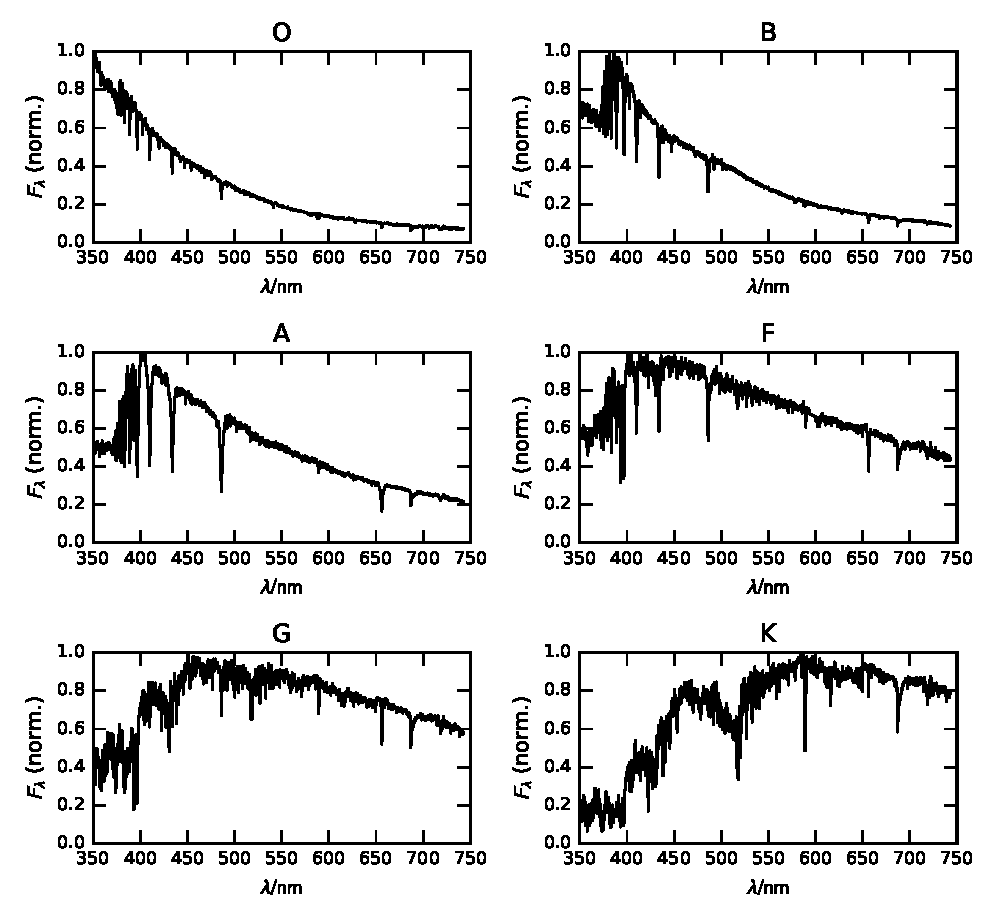
\includegraphics[width=\linewidth]{spectral_types}
\caption[Standard stellar types]{\label{f.spectral-types} Spectra from main-sequence stars of spectral types O--K. Data from \protect\citet{Jacoby1984A-library-of-st}.}
\end{figure*}

\subsection{Surface gravity}

As we have seen, the temperature of the stellar atmosphere determines which species are present and hence which lines are present. The width of the line conveys information about the pressure at the photosphere. To understand this, we need to digress briefly on the shape of the line.

Let's begin with a simple system: a mass $m$ attached to a spring with force constant $k$ as shown in Fig.~\ref{f.simple-spring}.

\begin{marginfigure}[-8\baselineskip]
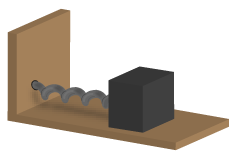
\includegraphics[width=\linewidth]{simple-spring}
\caption[A simple harmonic oscillator]{A simple harmonic oscillator: a mass $m$ on a frictionless surface attached to a  spring with force $F = -kx$.
\label{f.simple-spring}}
\end{marginfigure}

\subsection{With no driving force}

If we put the origin of our coordinate system where the mass is at rest with the spring relaxed, then the equation of motion of the mass is
\begin{equation}\label{e.SHO-basic}
	\DDtt{x} + \frac{k}{m} x = 0.
\end{equation}
You have solved this before: the most general solution is
\begin{equation}\label{e.SHO-general-solution}
	x(t) = x_{0}\cos(\wot) + \frac{v_{0}}{\omega_{0}}\sin(\wot)
\end{equation}
with $\omega_{0}^{2} = k/m$ and with $x_{0}$ and $v_{0}$ being the initial position and velocity of the mass.

\subsection{With driving at frequency $\omega \neq \omega_{0}$}

Now let's push on our mass with an oscillating force, $F\cos(\omega t)$ with $\omega\neq\omega_{0}$. A real world example would be holding a vibrating tuning fork near another fork tuned to a different frequency.  The equation of motion is now
\begin{equation}\label{e.SHO-driven}
	\DDtt{x} + \omega_{0}^{2}x = \frac{F}{m}\cos(\wt).
\end{equation}
You can verify by substitution that a general solution is
\[
	x(t) = \frac{F/m}{(\omega_{0}^{2}-\omega^{2})}\cos(\wt) + A\cos(\wot)+B\sin(\wot).
\]
Let's start with our harmonic oscillator at rest ($v_{0} = \left.\dif x/\dif t\right|_{t=0} = 0$) and at $\left. x\right|_{t=0} = 0$.  With these conditions, we can determine the constants $A$ and $B$; the solution is
\[
	x(t) = \frac{F/m}{(\omega_{0}^{2}-\omega^{2})}\left[\cos(\wt)-\cos(\wot)\right].
\]
Let's recast this by defining $\Delta = \omega_{0} - \omega$ and $\omega_{m} = (\omega_{0}+\omega)/2$.  Then
\begin{eqnarray*}
  \omega_{0}^{2}-\omega^{2} &=& (\omega_{0}-\omega)(\omega_{0}+\omega) = 2\Delta\omega_{m},\\
  \cos(\wot) &=& \cos\left(\wmt+\Delta t/2\right) = \cos(\wmt)\cos(\Delta t/2) - \sin(\wmt)\sin(\Delta t/2),\\
  \cos(\wt) &=& \cos\left(\wmt-\Delta t/2\right) = \cos(\wmt)\cos(\Delta t/2) + \sin(\wmt)\sin(\Delta t/2);
\end{eqnarray*}
and we write the solution as
\begin{equation}\label{e.beats}
	x(t) = \left[\frac{F/m}{\Delta\omega_{m}}\sin(\Delta t/2)\right]\sin(\wmt).
\end{equation}
This illustrates the phenomena of beats: the oscillation consists of a carrier signal at frequency $\omega_{m}$ with the amplitude modulated at the slower frequency $\Delta /2$.  Notice that the amplitude increases as $\Delta \to0$, i.e., $\omega\to\omega_{0}$.

\subsection{With both driving and damping}

Now let's make our model even more realistic by adding some damping.  We add a frictional force that is proportional to velocity, $F_{\mathrm{friction}} = -m\Gamma \dif x/\dif t$. Our complete equation of motion is then
\begin{equation}
	\DDtt{x} + \Gamma \DDt{x} + \omega_{0}^{2}x = \frac{F}{m}\cos(\omega t).
\end{equation}
The solution to this is straightforward to find, although the algebra is tedious (trust me on this). The general solution for initial conditions $\left.x\right|_{t=0} = x_{0}$ and $\left.\dif x/\dif t\right|_{t=0} = v_{0}$ is
\begin{eqnarray}
\label{e.general-solution-ddo}
\lefteqn{x(t) = \frac{F\womw/m}{\womw^{2}+\gw}\cos(\omega t)} && \\
	&+& \frac{\Gamma\omega F/m}{\womw^{2}+\gw}\sin(\omega t)\nonumber \\
	&+& \left[x_{0}-\frac{F\womw/m}{\womw^{2}+\gw}\right]{\color{red}e^{-\Gamma t/2}} \cos(\omega_{\Gamma}t) \nonumber\\
	&+& \left[\frac{v_{0}}{\omega_{\Gamma}}-\frac{\Gamma\omega F/m}{\womw^{2}+\gw}
	\,\frac{\omega}{\omega_{\Gamma}}\right]{\color{red}e^{-\Gamma t/2}} \sin(\omega_{\Gamma}t), 
	\nonumber
\end{eqnarray}
with
\[ 
    \omega_{\Gamma} = 
        \omega_{0}\left(1-\frac{\Gamma^{2}}{4\omega_{0}^{2}}\right)^{1/2}.
\]
Let's simplify this to the most relevant case.  First, the last two terms decay as {\color{red}$e^{-\Gamma t/2}$}: these are transients set by the initial conditions. After a time $2/\Gamma$ there will only be the first two terms, which oscillate at frequency $\omega$. 

We can simplify these first two terms even further: write
\[ \cos(\wt) = \frac{e^{i\wt}+e^{-i\wt}}{2},\quad \sin(\wt) 
    = \frac{e^{i\wt}-e^{-i\wt}}{2i}; \]
and combine terms to find
\begin{eqnarray}
    x(t) &=& \frac{F}{2m}\left[\frac{1}{\left(\omega_0^2-\omega^2\right) + i\Gamma\omega}\right]e^{i\wt} + \frac{F}{2m}\left[\frac{1}{\left(\omega_0^2-\omega^2\right) - i\Gamma\omega}\right]e^{-i\wt} \nonumber\\
    &=& \Re\left\{\frac{F}{m}\left[\frac{1}{\left(\omega_0^2-\omega^2\right) + i\Gamma\omega}\right]e^{i\wt}\right\}\label{e.oscillator-expression}
\end{eqnarray}
We use the symbol ``$\Re$'' to denote taking the real part of a complex quantity.  

From Eq.~(\ref{e.oscillator-expression}), we see that the oscillator can be described as the real part of a complex quantity $Ae^{i\wt}$, with
\[
    A = \frac{F}{m}\left[\frac{1}{\left(\omega_0^2-\omega^2\right) + i\Gamma\omega}\right].
\]
For $\omega \approx \omega_0$, we write $(\omega_0^2-\omega^2)\approx 2\omega_0(\omega_0-\omega)$ and take the square of the amplitude to find,
\begin{eqnarray}
    \left|A\right|^2 &=& \left(\frac{F}{2m\omega_0}\right)^2
        \frac{1}{(\omega_0-\omega)^2 + (\Gamma/2)^2}\nonumber\\
    &=& \frac{\pi}{2\Gamma}\left(\frac{F}{m\omega_0}\right)^2
        \left\{\frac{1}{\pi}\frac{\Gamma/2}{(\omega_0-\omega)^2 + (\Gamma/2)^2}\right\}
\end{eqnarray}
We rewrote the amplitude in the second line so that the term in $\{\cdot\}$ is normalized. The function
\[
    \mathcal{L}(\omega;\Gamma) = \frac{1}{\pi} 
        \frac{\Gamma/2}{(\omega_0-\omega)^2 + (\Gamma/2)^2}
\]
is known as a Lorentzian.  In contrast to a Gaussian, a Lorentzian is characterized by broad ``wings'' (Fig.~\ref{f.comparison}) as it goes to zero away from the central frequency $\omega_{0}$.
\begin{marginfigure}[-4\baselineskip]
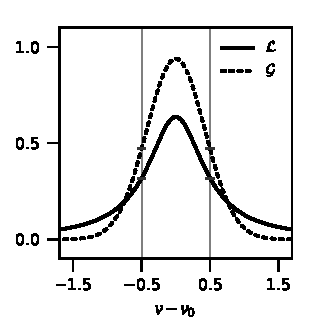
\includegraphics[width=\linewidth]{comparison}
\caption[Comparison of Lorentzian and Gaussian distributions]{\label{f.comparison}
Comparison of a Lorentzian ($\mathcal{L}$, solid line) and a Gaussian ($\mathcal{G}$, dotted line), both with $\mathrm{FWHM}=1$. The area under each curve is unity.}
\end{marginfigure}

\newthought{Consider an electronic transition in an atom between two energy levels, $E_m$ and $E_n$.} The natural frequency of this transition is $\nu_0 = |E_n-E_m|/h$. Light incident on the atom with frequency\sidenote{We are switching from angular frequency $\omega$ to frequency $\nu = \omega/2\pi$.} $\nu\neq\nu_0$ drives the electron at frequency $\nu$. An accelerating electron radiates, which damps the acceleration of the electron.  Classically, the transition in an atom is an electromagnetic oscillator with damping and driving terms, with cross-section\sidenote{For details, see the Box~\ref{b.line-emission}.}
\begin{equation}\label{e.semi-classical}
    \sigma = \left(\frac{\pi e^2}{m_e c}\right)
    \left\{\frac{\Gamma/4\pi}{(\nu_0-\nu)^2 + (\Gamma/4\pi)^2}\right\}.
\end{equation}
The actual value of the cross-section must be calculated using quantum mechanics. The overall shape of the cross-section is still in the form of equation~(\ref{e.semi-classical}) with opacity
\begin{equation}
    \rho\kappa_\nu = n_i \left(\frac{\pi e^2}{m_e c}\right) f_{mn}
        \left\{\frac{\Gamma/4\pi}{(\nu_0-\nu)^2 + (\Gamma/4\pi)^2}\right\}.
\end{equation}
In this equation, $f_{mn}$ is a number, called the \emph{oscillator strength}, that results from the calculation of the transition probability from state $m$ to state $n$, and $n_i$ is the density of atoms in state $m$.  The key point is that $f_{mn}$ depends only on the details of the transition: the energies, spins, and parities of the atomic states.  It does not depend on environmental parameters such as temperature and pressure.  As a result, $f_{mn}$ can be measured or computed once and then tabulated.


\begin{sidebar}[Treating line emission as a driven damped oscillator]
\label{b.line-emission}
NB. In this box, Gaussian CGS units are used for the electromagnetic field. To convert to MKS, make the following substitutions:
\begin{eqnarray*}
e &\to& \frac{1}{\sqrt{4\pi\varepsilon_0}}e\\
\bvec{E} &\to& \sqrt{4\pi\varepsilon_0}\bvec{E}\\
c &\to& (\mu_0\varepsilon_0)^{-1/2}.
\end{eqnarray*}

\newthought{Suppose we have a classical charged harmonic oscillator.}  The instantaneous power emitted by the oscillator is
\begin{equation}\label{e.larmor-power}
	 P(t) = \frac{2}{3}\frac{e^{2}}{c^{3}} |\dot{\vu}|^{2},
\end{equation}
and when averaged over a cycle is
\begin{equation}\label{e.oscillator-power}
	 \left\langle P(t) \right\rangle = \frac{e^{2}}{3c^{3}}x_{0}^{2} \omega^{4},
\end{equation}
since $\dot{\vu} = -\omega^{2}\bvec{x}_{0}\cos \omega t$. Since the oscillator is radiating, it is losing energy and is damped. Let us write the damping as $\bvec{F}_{\mathrm{rad}}\vdot \vu$; to find $\bvec{F}_{\mathrm{rad}}$, we integrate the power loss over a cycle,
\[  -\int_{t_{1}}^{t_{2}}\!\dif t\;\frac{2}{3}\frac{e^{2}}{c^{3}}\dot{\vu}\vdot\dot{\vu} 
	= -\left.\frac{2}{3}\frac{e^{2}}{c^{3}}\dot{\vu}\vdot\vu\right|_{t_{1}}^{t_{2}} 
	+ \frac{2}{3}\frac{e^{2}}{c^{3}} \int_{t_{1}}^{t_{2}}\!\dif t\;\ddot{\vu}\vdot\vu. 
\]
Since the motion is periodic, the first term vanishes and we can therefore identify 
\[ 
	\bvec{F}_{\mathrm{rad}} = \frac{2}{3}\frac{e^{2}}{c^{3}}\ddot{\vu} 
	= -m\left(\frac{2e^{2}\omega^{2}}{3c^{3}m}\right)\vu
\]
as the radiation damping term with the term in parenthesis being the damping constant $\gamma$. 
If there is an driving electric field on our oscillator, then its equation of motion becomes
\begin{equation}\label{e.eq-sho}
	m\ddot{\bvec{x}} = -m\omega_{0}^{2}\bvec{x} + e\bvec{E}e^{i\omega t} - m\gamma \dot{\bvec{x}}.
\end{equation}
Using a trial function $\bvec{x}\propto e^{i\omega t}$ gives
\[
	\bvec{x} = \frac{e}{m}\frac{E e^{i\omega t}}{(\omega_{0}^{2}-\omega^{2}) + i\omega\gamma}.
\]
Taking the second derivative w.r.t.\ time of $\bvec{x}$, substituting into eq.~(\ref{e.larmor-power}), and averaging over a cycle gives the power radiated by the oscillator,
\[
	\left\langle P(t)\right\rangle = \frac{e^{4}\omega^{4} E^{2}}{3 c^{2}m^{2}}
	\frac{1}{(\omega_{0}^{2}-\omega^{2})^{2} + \gamma^{2}\omega^{2}}.
\]
Dividing $\langle P(t)\rangle$ by the incident power per unit area, $cE^{2}/(8\pi)$, gives the cross-section:
\begin{equation}\label{e.classical-oscillator-cross-section}
	\sigma = \frac{8\pi}{3}\frac{e^{4}}{m^{2}c^{3}}
	\frac{\omega^{4}}{(\omega_{0}^{2}-\omega^{2})^{2} + \gamma^{2}\omega^{2}}.
\end{equation}
Now, for $\omega \approx \omega_{0}$, we can expand $(\omega_{0}^{2}-\omega^{2})^{2} \approx 4\omega_{0}^{2}(\omega_{0}-\omega)^{2}$; furthermore, we identify $2e^{2}\omega_{0}^{2}/(3c^{3}m) = \gamma$ and equation~(\ref{e.classical-oscillator-cross-section}) becomes
\begin{equation}\label{e.cross-section-lorentz}
	\sigma = \pi\left(\frac{e^{2}}{mc}\right)\frac{\gamma}{(\omega_{0}-\omega)^{2} + (\gamma/2)^{2}}.
\end{equation}
The line profile is Lorentzian, with a width $\gamma$. In terms of wavelength, the width is
\[ 
	\Delta \lambda = \left|\frac{\dif\lambda}{\dif\omega}\right|\gamma = \frac{2\pi c}{\omega^{2}}\gamma
	= \val{\sci{1.2}{-4}}{\textrm{\AA}}.
\]
This width is independent of the transition frequency (it is just the classical electron radius), and it is very, very small.  In a stellar atmosphere, the width is set by interactions and doppler broadening.

\newthought{To understand how impacts affect the line width}, suppose we model the oscillator as being started and stopped by impacts; in between impacts it just goes as $e^{i\omega_{0}t}$.  To get the spectrum, we take the Fourier transform,
\[
	F(\omega,t) = \int_{0}^{t}\!\dif t'\; \exp[i(\omega_{0}-\omega)t'],
\]
where $t$ is some time between impacts. Now if the impacts are distributed randomly and are uncorrelated, then the distribution of wait times follows a Poisson distribution,
\[ W(t)\,\dif t = e^{-t/\tau}\,\dif t/\tau, \]
where $\tau$ is the average time between collisions.  Using this to compute the energy spectrum, we obtain
\[ E(\omega) = \frac{1}{2\pi\tau}\int_{0}^{\infty}\!\dif t\; F(\omega,t)F^{*}(\omega,t)W(t) = \frac{1}{\pi\tau} 
	\frac{1}{(\omega_{0}-\omega)^{2} + (1/\tau)^{2}};
\]
the line profile is again Lorentzian, with a FWHM $2/\tau$.
\end{sidebar}

\newthought{There is an intrinsic width $\Gamma$ that is set by the finite lifetime of the energy levels;} in practice, however, this is not important.  In a stellar atmosphere, the width $\Gamma$ is set by collisions.  For example, when an electron passes close by our atom, the electric field shifts the energy levels of the atom\sidenote{This is an application of the \emph{Stark} effect that you learn about in quantum mechanics.}.  The greater the collision rate, the larger the width.
If we have two stars of the same photospheric temperature (so that both stars have the same lines), then a way to increase the collision rate is to increase the pressure. Recall, however, that in the stellar atmosphere $P = (g/\kappa)\tau$; as a result, stars with a higher surface gravity will have broader lines. The inset in Figure~\ref{f.compare_grav} illustrates the broadening of the Balmer H$\gamma$ line ($5\to 2$) in the spectrum of a main-sequence A1 star compared with that of a supergiant A1 star.

\begin{figure}[hp]
    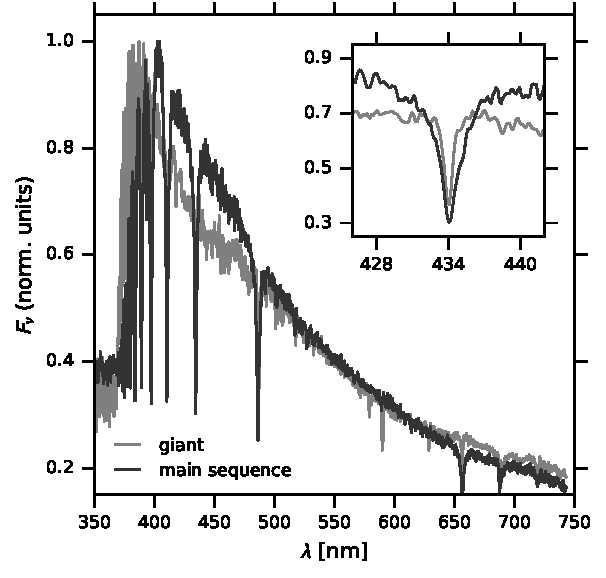
\includegraphics[width=\linewidth]{compare_grav}
    \caption[Spectra of two A1 stars]{\label{f.compare_grav}
    Spectra of two A1 stars, HD 16608 (a main sequence star) and SAO 12149 (a supergiant star).  Spectra are from \citet{Jacoby1984A-library-of-st}.
    }
\end{figure}

In addition to the width set by collisions, the line is also broadened by thermal motion: the atoms are in ceaseless motion; those headed towards us absorb at a blueshifted frequency, while those headed away from us absorb at a redshifted frequency.  Because the atomic velocities follow a Maxwell-Boltzmann distribution, the net effect is to make the core of the line (that is, near the center) assume a Gaussian profile.  Because a Gaussian falls off more quickly than a Lorentzian profile (see Fig.~\ref{f.comparison}), the wings of the line are still determined by the collision rate.

We might be inclined to treat the atoms as hard spheres, but this gives a large $\tau$, or equivalently a narrow line width. We are therefore led to consider longer-range interactions for setting the intrinsic line width. Table~\ref{t.perturbers} lists such interactions. For a given impact parameter, the interaction perturbs the energy levels; by integrating over a distribution of  impact parameters one gets the intrinsic damping. Of course, we should really use a quantum mechanical calculation.  We can scale our cross-section to the classical result (eq.~[\ref{e.cross-section-lorentz}]), however, by writing
\begin{equation}\label{e.cross-section}
	 \sigma_{\nu} = \left(\frac{\pi e^{2}}{m_{e}c}\right) f \phi_{\nu}, 
\end{equation}
where $\phi_{\nu}$ is the line profile (dimension $\sim \Hz^{-1}$) and $f$ is a dimensionless cross-section called the \newterm{oscillator strength}.

\begin{table}[htbp]
\caption{Interactions in stellar atmospheres}\label{t.perturbers}
\begin{tabular}{crcc}
\hline
perturbation & form & source & affects\\
\hline\hline
linear Stark & $C_{2} r^{-2}$ & $e^{-}$, $p$, ions & H (H$\alpha$, H$\beta$, \ldots)\\
quadratic Stark & $C_{4} r^{-4}$ & $e^{-}$ & non-hydrogenic ions\\
van der Waals & $C_{6}r^{-6}$ & atoms, H & most atomic lines, esp.\ in cool stars\\
\hline
\end{tabular}
\end{table}
